%&pdflatex
\documentclass[smallextended, referee]{svjour3} % svjour3: smallextended, referee
\usepackage[english]{babel}
\usepackage[T1]{fontenc}
\usepackage{graphicx}
\usepackage{amssymb, amsmath}
\usepackage{endfloat}
\usepackage{cite}
\usepackage{fixltx2e}
\usepackage{fullpage}

\newcommand{\Kn}{\mathrm{Kn}}
\newcommand{\dd}{\:\mathrm{d}}
\newcommand{\pder}[2][]{\frac{\partial#1}{\partial#2}}
\newcommand{\pderdual}[2][]{\frac{\partial^2#1}{\partial#2^2}}
\newcommand{\pderder}[3][]{\frac{\partial^2#1}{\partial#2\partial#3}}
\newcommand{\Pder}[2][]{\partial#1/\partial#2}

\journalname{Theoretical and Computational Fluid Dynamics}

\begin{document}

\title{
    Computer simulation of slightly rarefied gas flows driven by significant temperature variations and their continuum limit
}

\author{O.A.~Rogozin}
\institute{O.A.~Rogozin \at
    Moscow Institute of Physics and Technology,
    9 Institutskiy pereulok, g. Dolgoprudny,
    Moskovskaya obl., Russian Federation\\
    \email{o.a.rogozin@gmail.com}
}

\maketitle

\begin{abstract}
    Classical fluid dynamics describes the behavior of gas in terms of the Navier--Stokes equations.
    However, a rigorous asymptotic analysis of the Boltzmann equation for small Knudsen numbers
    restricts the scope of its application and leads, in the general case,
    to more complicated sets of differential equations.
    The present paper deals with the one which is valid for significant
    temperature variations and finite Reynolds numbers.
    A special-purpose solver on the open-source CFD platform OpenFOAM\textregistered{} is proposed
    for computer simulation of a slightly rarefied gas in an arbitrary geometry.
    Several temperature driven flows are considered as examples.
    \keywords{
        OpenFOAM \and
        Boltzmann equation \and
        Navier--Stokes equations \and
        thermal creep flow \and
        nonlinear thermal-stress flow \and
        ghost effect
    }
    \PACS{47.45.-n,47.11.Df}
\end{abstract}

\section{Introduction}

%%% Current state of affairs
The Navier--Stokes equations are widely used for modeling of a gas with the vanishing mean free path.
Slightly rarefied gas effects, which are widely thought to take place only in the thin Knudsen layer,
can be taken into account using the slip conditions on the boundary~\cite{SharipovCoefficients}.
In some situations, however, the Navier--Stokes set fails to describe the correct density and temperature fields
even in the continuum limit~\cite{Kogan1976, GhostEffect}.
When the Reynolds number is finite and the temperature variations are large:
\[ \mathrm{Re} = O(1), \quad \frac1T\left|\pder[T]{x_i}\right| = O(1), \]
higher-order terms of gas rarefaction begin to play a significant role in the gas behavior.
In this case, the asymptotic analysis of the Boltzmann equation arrives on the scene and
yields the appropriate equations on the macroscopic variables, together with
their associated boundary conditions~\cite{Sone2002, Sone2007}.

%%% Existing solutions
This new set of equations has the similar structure to the Navier--Stokes one,
so similar numerical methods can be utilized too.
The pioneering solutions are based on the finite difference methods~\cite{GhostEffect, Kogan1976}.
The finite volume method is applied in some recent works~\cite{Laneryd2006, Laneryd2007}.

%%% Limitations
Currently, many CFD platforms provide comprehensive
capabilities for numerical simulation of the Navier--Stokes equations,
but the considered fluid-dynamic-type set of equations remains in the shadow.
The goal of the present paper is to improve this situation and
draw more attention to such CFD scope extensions.

%%% Why OpenFOAM?
One of the modern and promising CFD platforms, OpenFOAM\textregistered{},
has been selected as a basis for numerical algorithms developing.
OpenFOAM\textregistered{} is an object-oriented C++ library of classes and routines for parallel computation,
providing a set of high-level tools for writing advanced CFD code~\cite{OpenFOAM1998}.
It has a wide set of basic features, similar to any commercial one~\cite{OpenFOAM2010},
and is a robust and reliable software widely used in the industry~\cite{BoilingFlows2009,
TurbulentCombustion2011, CoastalEngineering2013, BiomassPyrolysis2013}.
As for rarefied gas, OpenFOAM\textregistered{} has a standard solver for DSMC, that
can be extended for hybrid simulations~\cite{HybridSolver2012}.
Finally, the most important advantage of OpenFOAM\textregistered{} is its open-source code,
so it is easy to add any modification to any part of the implementation.
OpenFOAM\textregistered{} is also well documented and has a large and active community of users.

\section{Basic equations}

The behavior of a gas is governed by the conservation equations of mass, momentum, and energy:
\begin{gather}
    \pder[\rho]{t} + \pder{x_i}(\rho v_i) = 0, \label{eq:mass}\\
    \pder{t}(\rho v_i) + \pder{x_j}(\rho v_i v_j + p_{ij}) = \rho F_i, \label{eq:momentum}\\
    \pder{t}\left[\rho\left(e+\frac{v_i^2}2\right)\right]
        \pder{x_j}\left[\rho v_j\left(e+\frac{v_i^2}2\right)+v_i p_{ij}+q_j\right] = \rho v_j F_j. \label{eq:energy}
\end{gather}
Macroscopic variables have the following notation: the density \(\rho\), the flow velocity \(v_i\),
the stress tensor \(p_{ij}\), the specific internal energy \(e\), and the heat-flow vector \(q_i\).
Finally, \(F_i\) denotes the external force.
For an ideal monatomic gas, the internal energy \(e = 3RT/2\) depends only on the temperature;
\(R = k_B / m\) is the specific gas constant.
The pressure is taken from the equation of state \( p = \rho RT \).

The Navier--Stokes set equations is obtained from the conservation equations with the help of Newton's law,
\begin{equation}\label{eq:Newton_law}
    p_{ij} = p\delta_{ij} - \mu\left(\pder[v_i]{x_j}+\pder[v_j]{x_i}-\frac23\pder[v_k]{x_k}\delta_{ij}\right) -
        \mu_B\pder[v_k]{x_k}\delta_{ij},
\end{equation}
and Fourier's law,
\begin{equation}\label{eq:Fourier_law}
    q_i = -\lambda\pder[T]{x_i}.
\end{equation}
Some of the transport coefficients are used here:
the viscosity \(\mu\), the bulk viscosity \(\mu_B\), and the thermal conductivity \(\lambda\).
The bulk velocity of an ideal monoatomic gas is zero (\(\mu_B = 0\)).

The Knudsen number \(\Kn = \ell/L\), the parameter characterizing the rate of rarefaction of the gas,
is determined by the ratio of the mean free path \[ \ell = \frac{m}{\sqrt2\pi d_m^2 \rho} \]
to the reference length \(L\).
For a hard-sphere gas, the radius of the influence range of the intermolecular force \(d_m\)
coincides with the diameter of a molecule.
The viscosity \(\mu\) and the thermal conductivity \(\lambda\) of an ideal gas
are proportional to the mean free path \(\ell\) and therefore to the Knudsen number:
\begin{equation}
    \mu = O(\Kn), \quad \lambda = O(\Kn).
\end{equation}

In the continuum limit (\(\Kn\to0\)), we obtain the Euler set of equations where
\begin{equation}
    p_{ij} = p\delta_{ij}, \quad q_i = 0
\end{equation}
that makes it impossible to determine the temperature field of a gas at rest.
The classical heat-conduction equation
can be derived from~\eqref{eq:energy} and~\eqref{eq:Fourier_law}
in the absence of gas flows (\(v_i = 0\)):
\begin{equation}\label{eq:heat_equation}
    \pder{x_i}\left(\sqrt{T}\pder[T]{x_i}\right) = 0.
\end{equation}
Here, it is taken into account that the thermal conductivity of a hard-sphere gas
is proportional to \(\sqrt{T}\).

A rigorous examination of the continuum limit shows that the infinitesimal thermal conduction term \(\Pder[q_j]{x_j}\)
can be of the same order as the thermal convective term \(\Pder[pv_j]{x_j}\) in the energy equation~\eqref{eq:energy}.
In such a case, when the Mach number is the same order of as the Knudsen number,
the heat-conduction equation~\eqref{eq:heat_equation} fails to describe
the correct temperature field. Moreover, additional thermal stress terms of the second order of \(\Kn\)
appears in the momentum equation~\eqref{eq:momentum}.
These important modifications can be systematically considered only within the scope of kinetic theory.

\section{Asymptotic analysis of the Boltzmann equation}

A detailed mathematical derivation of the results introduced in this section
can be found in~\cite{Sone2002, Sone2007}.

Unless explicitly otherwise stated, all variables are further assumed to be dimensionless
by taking the following reference quantities:
the length \(L\), the pressure \(p^{(0)}\), the temperature \(T^{(0)}\),
the velocity \((2RT^{(0)})^{1/2}\), the heat-flow vector \(p^{(0)}(2RT^{(0)})^{1/2}\),
and the external force \(2RT^{(0)}/L\).
It is also convenient to deal with the modified Knudsen number
\[ k = \frac{\sqrt\pi}2\frac{\ell^{(0)}}{L} = \frac{m}{2\sqrt{2\pi} d_m^2 \rho^{(0)}L}. \]

\subsection{Fluid-dynamic-type equations}

The analysis presented below is based on the conventional Hilbert expansion
of the distribution function \(f\) and macroscopic variables \(h\)~\cite{Hilbert1912}:
\[ f = f_0 + f_1k + f_2k^2 + \cdots, \quad h = h_0 + h_1k + h_2k^2 + \cdots \]
under the additional assumption
\begin{equation}\label{eq:Mach_constraint}
    u_i = O(k)
\end{equation}
means that the Mach number is of the same order as the Knudsen number.
Moreover, let the external force be weak:
\begin{equation}\label{eq:Force_constraint}
    F_i = O(k^2).
\end{equation}
Conditions~\eqref{eq:Mach_constraint} and~\eqref{eq:Force_constraint} make the pressures
\(p_0\) and \(p_1\) constant due to the degenerated momentum equation~\eqref{eq:momentum}:
\begin{equation}
    \pder[p_0]{x_i} = 0, \quad \pder[p_1]{x_i} = 0.
\end{equation}

Then, the following set of equations for a time-independent case (\(\Pder{t} = 0\))
is obtained for variables \(T_0\), \(u_{i1} = p_0v_{i1}\), \(p_2^\dag\):
\begin{align}
    \pder{x_i}\left(\frac{u_{i1}}{T_0}\right) &= 0, \label{eq:asymptotic1} \\
    \pder{x_j}\left(\frac{u_{i1}u_{j1}}{T_0}\right)
        &-\frac{\gamma_1}2\pder{x_j}\left[\sqrt{T_0}\left(
            \pder[u_{i1}]{x_j} + \pder[u_{j1}]{x_i} - \frac23\pder[u_{k1}]{x_k}\delta_{ij}
        \right)\right] \notag\\
        &- \frac{\gamma_7}{T_0}\pder[T_0]{x_i}\pder[T_0]{x_j}\left(\frac{u_{j1}}{\gamma_2\sqrt{T_0}} - \frac{1}4\pder[T_0]{x_j}\right) \notag\\
        &= -\frac{p_0}{2}\pder[p_2^\dag]{x_i} + \frac{p_0^2 F_{i2}}{T_0}, \label{eq:asymptotic2} \\
    \pder[u_{i1}]{x_i} &= \frac{\gamma_2}2\pder{x_i}\left(\sqrt{T_0}\pder[T_0]{x_i}\right), \label{eq:asymptotic3}
\end{align}
where
\begin{equation}\label{eq:dag_pressure}
    p_2^\dag = p_2
        + \frac{2\gamma_3}{3p_0}\pder{x_k}\left(T_0\pder[T_0]{x_k}\right)
        - \frac{\gamma_7}{6p_0}\left(\pder[T_0]{x_k}\right)^2.
\end{equation}
The set of equations \eqref{eq:asymptotic1}--\eqref{eq:asymptotic3} has a fluid-dynamic nature
and is comparable to the Navier--Stokes equations for a compressible gas (\(\rho_0 = p_0/T_0\)).
The formal difference consists in the additional thermal stress term.
Comparing it with \(p_0^2F_{i2}/T_0\), we find that
\begin{equation}\label{eq:force}
    k^2\frac{\gamma_7}{p_0^2}\pder[T_0]{x_i}\pder[T_0]{x_j}\left(\frac{u_{j1}}{\gamma_2\sqrt{T_0}} - \frac{1}4\pder[T_0]{x_j}\right)
\end{equation}
is the force acting on unit mass of the gas.
For a hard-sphere gas at rest, this force is opposite to the temperature gradient direction.

It should be noted that \(p_2^\dag\) is not included in the equation of state and
therefore is determined up to a constant factor.
Term \(\Pder[p_2^\dag]{x_i}\) participates in the system as the pressure
in the Navier--Stokes set for an incompressible gas.
This fact specifies the class of suitable numerical methods
for solving \eqref{eq:asymptotic1}--\eqref{eq:asymptotic3}.

For a hard-sphere gas, the transport coefficients are
\begin{alignat*}{2}
    \gamma_1 &= 1.270042427, &\quad \gamma_2 &= 1.922284066, \\
    \gamma_3 &= 1.947906335, &\quad \gamma_7 &= 1.758705.
\end{alignat*}
The first two are connected to the dimensional transport coefficients in the following way:
\begin{equation}
    \mu = \gamma_1\sqrt{T_0} \frac{p^{(0)}L}{\sqrt{2RT^{(0)}}} k, \quad
    \lambda = \frac{5\gamma_2}{2}\sqrt{T_0} \frac{p^{(0)}RL}{\sqrt{2RT^{(0)}}} k,
\end{equation}
and \(\gamma_7\) is related to the \emph{nonlinear thermal-stress flow}.
Other molecular models are easily applied by replacing these coefficients.
Appropriate formulas for their numerical evaluation can be found in~\cite{GhostEffect, Sone2002, Sone2007}.

The stress tensor and the heat-flow vector are obtained as follows:
\begin{alignat*}{2}
    p_{ij0} &= p_0\delta_{ij}, && \quad q_{i0} = 0, \\
    p_{ij1} &= p_1\delta_{ij}, && \quad q_{i1} = -\frac{5\gamma_2}4\sqrt{T_0}\pder[T_0]{x_i}, \\
    p_{ij2} &= p_2\delta_{ij}
                &&- \frac{\gamma_1}{p_0}\sqrt{T_0}\left(
                \pder[u_{i1}]{x_j} + \pder[u_{j1}]{x_i} - \frac23\pder[u_{k1}]{x_k}\delta_{ij}
            \right) \\
        & &&+ \frac{\gamma_3}{p_0} T_0\left(
                \pderder[T_0]{x_i}{x_j} - \frac13\pderdual[T_0]{x_k}\delta_{ij}
            \right) \\
        & &&+ \frac{\gamma_7}{p_0}\left[
                \pder[T_0]{x_i}\pder[T_0]{x_j} - \frac13\left(\pder[T_0]{x_k}\right)^2\delta_{ij}
            \right].
\end{alignat*}

\subsection{Boundary conditions}

The fluid-dynamic boundary conditions based on the diffuse-reflection boundary conditions
for Boltzmann equation look as follows:
\begin{gather}
    T_0 = T_B, \label{eq:bound:T} \\
    \left\{
    \begin{aligned}
        & \frac{(u_{j1}-u_{Bj1})}{\sqrt{T_B}}(\delta_{ij}-n_in_j) =
            -K_1\pder[T_B]{x_j}(\delta_{ij}-n_in_j), \\
        & u_{j1}n_j = 0.
    \end{aligned}
    \right. \label{eq:bound:v}
\end{gather}
Here, \(n_i\) is the unit normal vector to the boundary, pointing into the gas.
\(u_{Bj1}\) is the velocity of the boundary, and \(T_B\) is its temperature.
\(K_1\) is the slip coefficient related to the \emph{thermal creep flow}.
For a hard-sphere gas, \[ K_1 = -0.6463. \]
Thus, the direction of the thermal creep flow coincides with the temperature gradient.

The solution of the boundary-value problem cannot be expressed in terms of the fluid-dynamic-type
solution due to the sharp variation in the distribution function near the boundary.
Therefore, it is necessary to introduce the so-called Knudsen-layer correction:
\begin{equation}
    f = f_{FD} + f_K, \quad h = h_{FD} + h_K.
\end{equation}
The fluid-dynamic part \(f_{FD}\) is the solution presented above,
and \(f_K\) decays exponentially with the distance to the boundary \(f_K = O\left(e^{-\eta}\right)\).
The relation \( x_i = k\eta n_i(s_1,s_2) + x_{Bi}(s_1, s_2) \) gives a coordinate transformation
from \((x_1,x_2,x_3)\) to \((\eta,s_1,s_2)\).

Due to the infinitesimal Mach number~\eqref{eq:Mach_constraint}, \(f_K\) is expanded
in a power series of \(k\), starting from the first order:
\[ f_K = f_{K1} k + f_{K2} k ^ 2 + \cdots \]
The Knudsen layer introduces a correction to \(u_{i1}\) for a hard-sphere gas:
\begin{equation}
    \left\{
    \begin{aligned}
        & \frac{u_{jK1}}{\sqrt{T_B}}(\delta_{ij}-n_in_j) =
            -\frac12\pder[T_B]{x_j} Y_1\left(\frac\eta{T_B}\right) (\delta_{ij}-n_in_j), \\
        & u_{jK1}n_j = 0.
    \end{aligned}
    \right. \label{eq:bound:v_K}
\end{equation}
The function \(Y_1(\eta)\) is tabulated, for example, in~\cite{Sone2002, Sone2007} and is shown in Fig.~\ref{fig:Y1}.

\begin{figure}[ht]
    \centering
    \begin{minipage}{.48\textwidth}
        \centering
        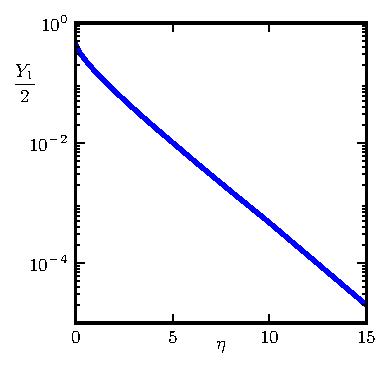
\includegraphics{Fig1}
        \caption{The function of the Knudsen layer \(Y_1(\eta)/2\) for a hard-sphere gas.}
        \label{fig:Y1}
    \end{minipage}
    \quad
    \begin{minipage}{.48\textwidth}
        \centering
        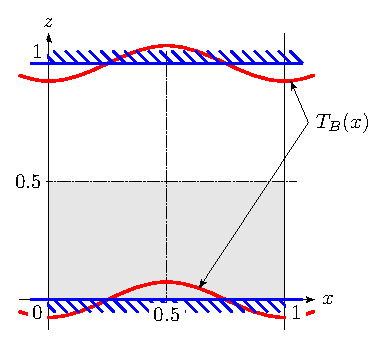
\includegraphics{Fig2}
        \vspace{13pt}
        \caption{Geometry of the problem: the gas is placed between two parallel plates
            with the periodical temperature distribution \(T_B\).}
        \label{fig:geometry}
    \end{minipage}
\end{figure}

\subsection{Some remarks on the continuum limit}

As one can see from~\eqref{eq:asymptotic3}, a gas is not always described correctly
by the heat-conduction equation~\eqref{eq:heat_equation}.
Equation~\eqref{eq:asymptotic3} converges to~\eqref{eq:heat_equation} if \(u_{i1} = 0\).
In the absence of an external force, there are several reasons when this condition can be violated:
\begin{enumerate}
    \item The boundary is moving: \(u_{B1i} \neq 0 \).
    \item The boundary temperature is not uniform: \(\Pder[T_B]{x_i} \neq 0 \).
    \item The isothermal surfaces are not parallel:
        \begin{equation}\label{eq:equilibrium}
            e_{ijk}\pder[T_0]{x_j}\pder{x_k}\left(\pder[T_0]{x_l}\right)^2 \neq 0.
        \end{equation}
\end{enumerate}
The first two cases are directly determined by the boundary conditions,
and the third one has only an implicit impact from them.

The set of equations~\eqref{eq:asymptotic1}--\eqref{eq:asymptotic3} revealed the following interesting fact.
In the continuum limit, the velocity field tends to zero, proportional to the Knudsen number,
due to~\eqref{eq:Mach_constraint}, however infinitesimally weak flows
have a finite impact on the temperature field.
Such an asymptotic behavior of a system of differential equations
is called the \emph{ghost effect}~\cite{GhostEffect, Sone2002, Sone2007}.

\section{Numerical simulation and discussions}

\begin{figure}[ht]
    \centering
    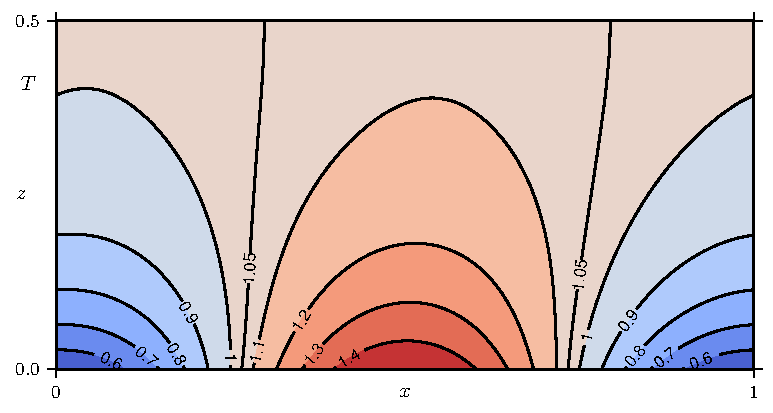
\includegraphics{Fig3}
    \caption{The temperature field \(T_0\) obtained from the asymptotic theory:
        isothermal lines are placed above the contour lines.}
    \label{fig:moving:T_asym}
\end{figure}

\begin{figure}[ht]
    \centering
    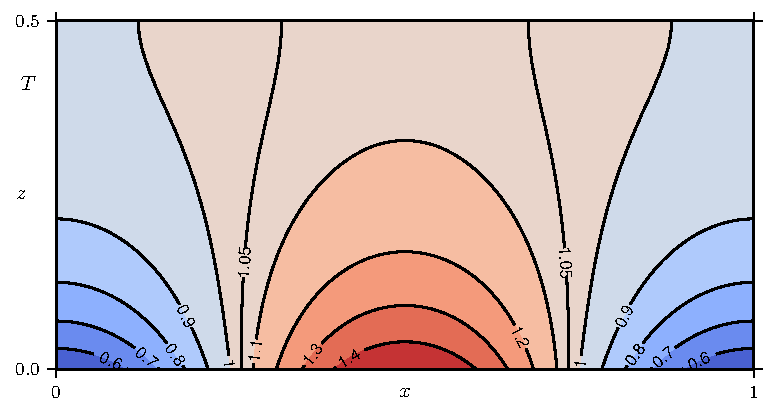
\includegraphics{Fig4}
    \caption{Temperature field \(T\) obtained from the heat-conduction equation:
        isothermal lines are placed above the contour lines.}
    \label{fig:moving:T_heat}
\end{figure}

The present results are obtained with the special solver of the system~\eqref{eq:asymptotic1}--\eqref{eq:asymptotic3}.
It has been developed within the open-source CFD toolbox OpenFOAM\textregistered{}~\cite{OpenFOAM1998},
based on the finite-volume approach for evaluating partial derivatives.
The continuity equation~\eqref{eq:asymptotic1}, along with the momentum equation~\eqref{eq:asymptotic2},
is solved with the commonly used implicit conservative SIMPLE algorithm~\cite{SIMPLE}.
A detailed description of this scheme for gas mixtures can be found in~\cite{Laneryd2007}.

Unstructured spatial grids are generated with the open-source package GMSH~\cite{GMSH}.
They are nonuniform and condensed in areas with large gradients of macroscopic variables.
From \(10^3\) to \(10^6\) cells are used to achieve the residual of the solution
that is not greater than \(10^{-6}\) for all considered problems.

OpenFOAM\textregistered{} uses Kitware's ParaView\textregistered{} as a primary visualization system of results,
but for the present paper another open-source tool, Matplotlib, has been chosen to create color vector illustrations.

All transport coefficients are taken in compliance with the hard-sphere model.
Complete diffuse reflection is assumed from a solid boundary.
The external force is taken to be zero.

\subsection{Gas between two parallel plates}

Consider a plane periodic geometry shown in Fig.~\ref{fig:geometry}.
A gas is placed between two infinite parallel plates
both have a periodic distribution of the temperature and the small velocity
\begin{equation}
    T_B = 1-\alpha\cos(2\pi x), \quad u_{Bi} = (\beta\Kn,0,0).
\end{equation}
Due to the symmetry, the computational domain represents a rectangle \(0<x<1, 0<z<1/2\)
(a gray background in Fig.~\ref{fig:geometry}).
The problem is simulated for
\[ \alpha=1/2, \quad \beta = 1 \]
to compare with the reference solution in~\cite{GhostEffect}.
Complete agreement between these results is a good verification of the solver validity.

\begin{figure}
    \centering
    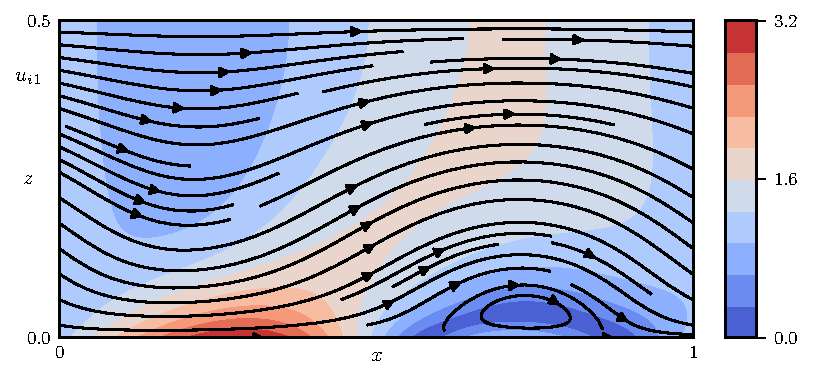
\includegraphics{Fig5}
    \caption{The fluid-dynamic part of the velocity field \(u_{FDi1}\):
        curves with arrows indicate the direction, contour lines show the magnitude.}
    \label{fig:moving:fluid}
\end{figure}

\begin{figure}
    \centering
    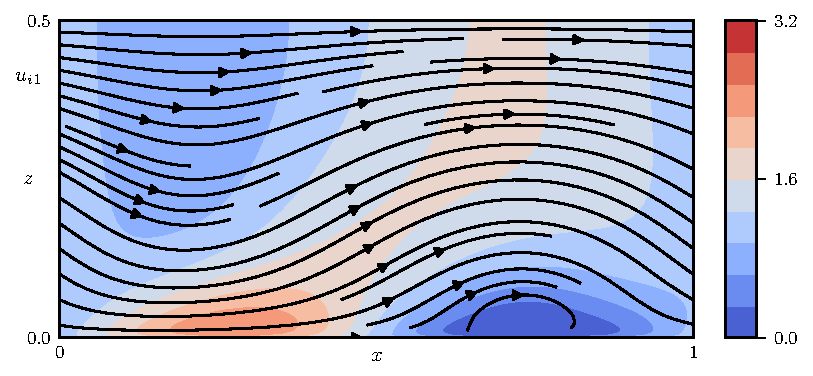
\includegraphics{Fig6}
    \caption{The velocity field \(u_{i1}\) with the Knudsen layer correction for \(\Kn=0.01\):
        curves with arrows indicate the direction, contour lines show the magnitude.}
    \label{fig:moving:kn001}
\end{figure}

The temperature field (Fig.~\ref{fig:moving:T_asym}) is shown
in comparison with the solution of the heat-conduction equation (Fig.~\ref{fig:moving:T_heat}).
In the continuum limit, \(T=T_0\), so we can see that the classical fluid-dynamic solution
has a finite distinction from the kinetic one.

The velocity field \(u_{i1}\) is shown in Fig.~\ref{fig:moving:fluid} and Fig.~\ref{fig:moving:kn001}.
The Knudsen layer correction~\eqref{eq:bound:v_K} is taken into account in the latter figure.
For small \(k\), a gas flow along the boundary temperature gradient occurs
in the thin Knudsen layer. This flow, which is of the first order of \(k\), is called
the \emph{thermal creep flow}.

\subsection{Gas between two cylinders and spheres}

\begin{figure}
    \centering
    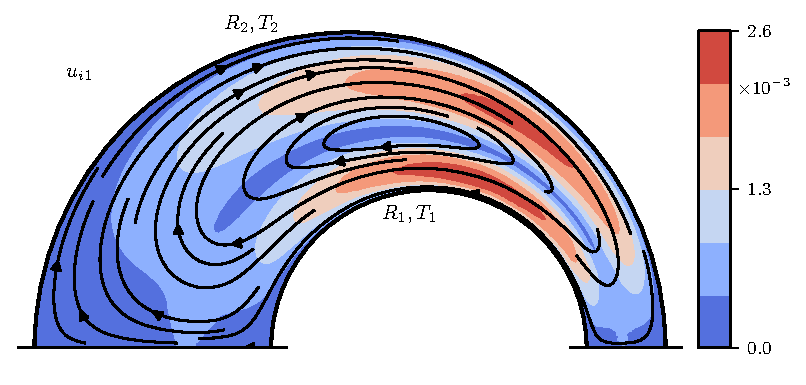
\includegraphics{Fig7}
    \caption{The velocity field \(u_{i1}\) between two noncoaxial cylinders:
        curves with arrows indicate the direction, contour lines show the magnitude.}
    \label{fig:cylinders}
\end{figure}

\begin{figure}
    \centering
    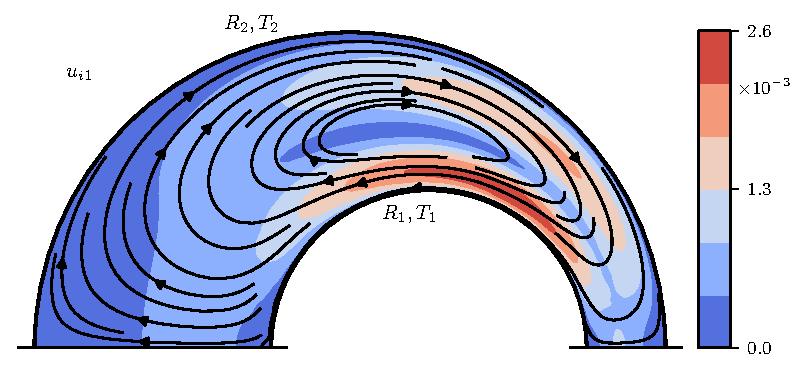
\includegraphics{Fig8}
    \caption{The velocity field \(u_{i1}\) between two nonconcentric spheres:
        curves with arrows indicate the direction, contour lines show the magnitude.}
    \label{fig:spheres}
\end{figure}

Now, consider the case, where there is no temperature gradient on the surface of the surrounding bodies at rest.
The Navier--Stokes equations with any slip boundary conditions have a trivial solution \(u_i = 0\)
that is, however, not valid for~\eqref{eq:asymptotic1}--\eqref{eq:asymptotic3}.
As stated above, even under such boundary conditions, a convection flow can emerge
due to nonparallelism of the isothermal surfaces~\eqref{eq:equilibrium}.
This phenomenon is called the \emph{nonlinear thermal-stress flow}
and is described first in~\cite{Kogan1971} in terms of the Chapman--Enskog expansion
that gives the similar equations to~\eqref{eq:asymptotic1}--\eqref{eq:asymptotic3}
but with slightly different transport coefficients.
The nonlinear origin of this effect in the first order of the Knudsen number is relevant,
because a linear thermal-stress flow appears only in the following order of smallness \(O(k^2)\).
This type of convection has an important feature. It can occur in the state of weightlessness
whereas a gas convection in the classical sense can be driven only by a finite external force.
Some experimental studies of the nonlinear thermal-stress flow can be found in~\cite{ExperimentsNTFS2003}.

Consider two cylinders of radius \(R_1 = 1\) and \(R_2 = r\)
with temperatures \(T_1 = 1\) and \(T_2 = \alpha\), respectively.
The cylinder axes are parallel; the distance between them is equal to \(d\).

Fig.~\ref{fig:cylinders} presents the results of the numerical simulation for
\[ r = 2, \quad d = 1/2, \quad \alpha = 2. \]
The velocity field \(u_{i1}\) for this problem is much weaker than in the previous example,
so it has too small influence on the temperature distribution that we skip to demonstrate.
A gas between nonconcentric spheres is also simulated in the same geometry (Fig.~\ref{fig:spheres}).

\subsection{Gas between two elliptical cylinders}

\begin{figure}
    \centering
    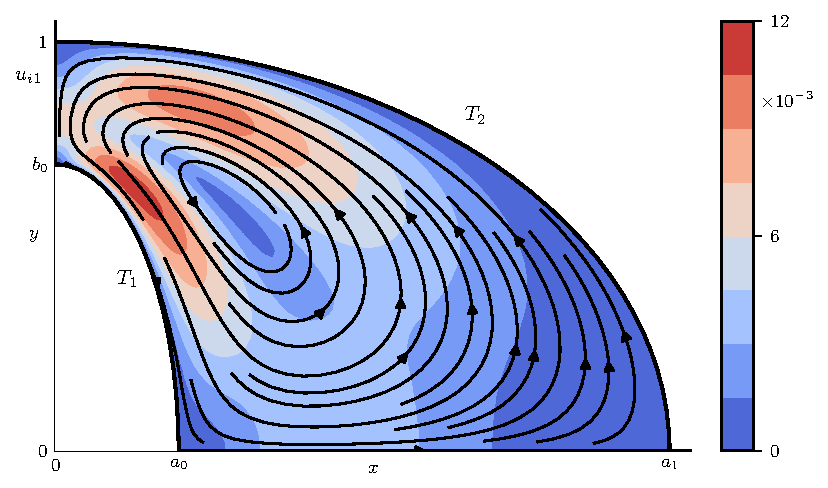
\includegraphics{Fig9}
    \caption{The velocity field \(u_{i1}\) between coaxial elliptical cylinders:
        curves with arrows indicate the direction, contour lines show the magnitude.}
    \label{fig:elliptic}
\end{figure}

In the last example, a gas is placed between two coaxial elliptical cylinders
in such a way that the major axes of the ellipses are perpendicular in a cross section.
Let the semi-minor axis of the outer cylinder be the characteristic length, while the semi-major one is \(a_1\).
The semi-axes of the inner ellipse are \(a_0\) and \(b_0\) in length.
The temperatures are \(T_1 = 1\) and \(T_2 = \alpha\) again.

In Fig.~\ref{fig:elliptic} the velocity field is shown for
\[ a_1 = 1.5, \quad a_0 = 0.3, \quad b_0 = 0.7, \quad \alpha = 2. \]
Numerical simulation of a rarefied gas using the DSMC method in the same geometry
for a wide range of Knudsen numbers \(0.1\le\Kn\le5\) can be found in~\cite{SoneCoaxial}.

\begin{figure}[ht]
    \centering
    \begin{minipage}{.48\textwidth}
        \centering
        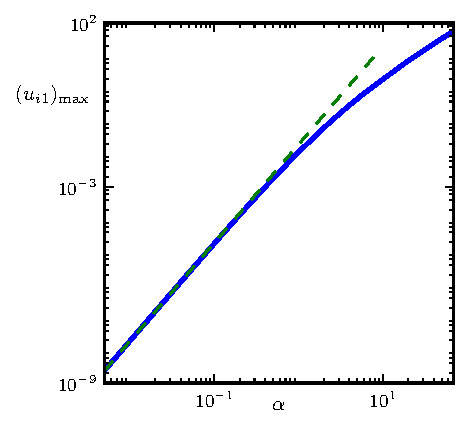
\includegraphics{Fig10}
        \caption{The maximum magnitude of \(u_{i1}\) versus the temperature ratio of the cylinders \(\alpha\).
            The dashed line corresponds the cubic relation.}
        \label{fig:maxU}
    \end{minipage}
    \quad
    \begin{minipage}{.48\textwidth}
        \centering
        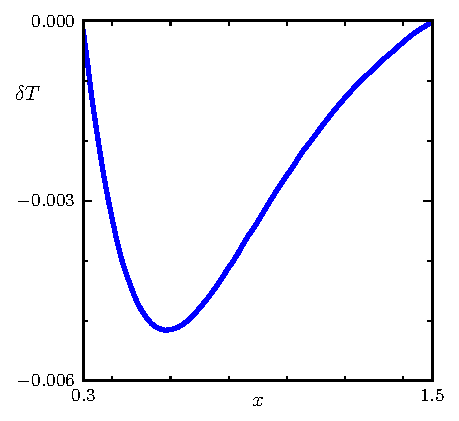
\includegraphics{Fig11}
        \caption{Difference between temperature distributions \(\delta T\) of the heat-conduction equation
            and the asymptotic theory along the \(x\) for \(\alpha = 5\).}
        \label{fig:deltaT}
    \end{minipage}
\end{figure}

A calculation of presented problems on the modern personal computer (3.40GHz CPU)
takes about several minutes for the most detailed spacial grids.
This fact provides a great performance for parametric studies as well. As an example,
the maximum magnitude of \(u_{i1}\) as a function of \(\alpha\) is shown in Fig.~\ref{fig:maxU}.
For small \(\alpha\),
\begin{equation}
    \mathrm{max}(u_{i1}) \propto \alpha^3, \quad \alpha\to0.
\end{equation}

Finally, Fig.~\ref{fig:deltaT} illustrates the discrepancy between the temperature fields
obtained from the asymptotic theory and the heat-conduction equation
\( \delta T = T_\mathrm{asym} - T_\mathrm{heat} \)
along the major axis of the outer cylinder.

\section{Conclusion}

%%% What it has been shown and achieved?
In the present paper, OpenFOAM\textregistered{}, a free and open-source CFD platform,
widely used and rapidly extending, is upgraded to deal with
slightly rarefied gas flows driven by significant temperature variations.
A reliable and rapid solver has been introduced on the basis of the appropriate
equations and boundary conditions, derived from the asymptotic analysis of the Boltzmann equation.
The program code has been validated by means of some benchmark simulations,
presented as illustrations. Typical problems of the first order of Knudsen number
have been considered: thermal creep flow and nonlinear thermal-stress flow.

%%% The meaning for the field
OpenFOAM\textregistered{}, together with the newly implemented numerical algorithm,
is a robust tool for numerical analysis of slightly rarefied gas problems
on the kinetic basis. The principal advantage of the developed code is that
it is easily extensible as an open-source software.

%%% Possible applications and extensions
A hard-sphere gas with the diffuse-reflection boundary condition is considered in this paper,
but various molecular models and boundary conditions can be used as well.
In addition, appropriate equations for gas mixtures can be also naturally implemented.

\bibliographystyle{spphys} % spbasic, spmpsci, spphys
\bibliography{springer}

\end{document}


